\documentclass{beamer}
%
% Choose how your presentation looks.
%
% For more themes, color themes and font themes, see:
% http://deic.uab.es/~iblanes/beamer_gallery/index_by_theme.html
%
\mode<presentation>
{
  \usetheme{default}      % or try Darmstadt, Madrid, Warsaw, ...
  \usecolortheme{default} % or try albatross, beaver, crane, ...
  \usefonttheme{default}  % or try serif, structurebold, ...
  \setbeamertemplate{navigation symbols}{}
  \setbeamertemplate{caption}[numbered]
} 

\usepackage[english]{babel}
\usepackage[utf8]{inputenc}
\usepackage{bm}
\usepackage{biblatex}
\usepackage{bibentry}
\addbibresource{poster.bib}
\setbeamertemplate{bibliography item}{}




\title[Your Short Title]{\Huge Latent Dirichlet Allocation}
\author{\Large Patrice B\'echard \quad Th\'eophile Gervet}
\institute{\normalsize Universit\'e de Montr\'eal}
\date{\Large \today}

\begin{document}

%
% Title page
%

\begin{frame}
  \titlepage
\end{frame}

%
% LDA figure
%

\begin{frame}{Context}
\noindent\makebox[\textwidth]{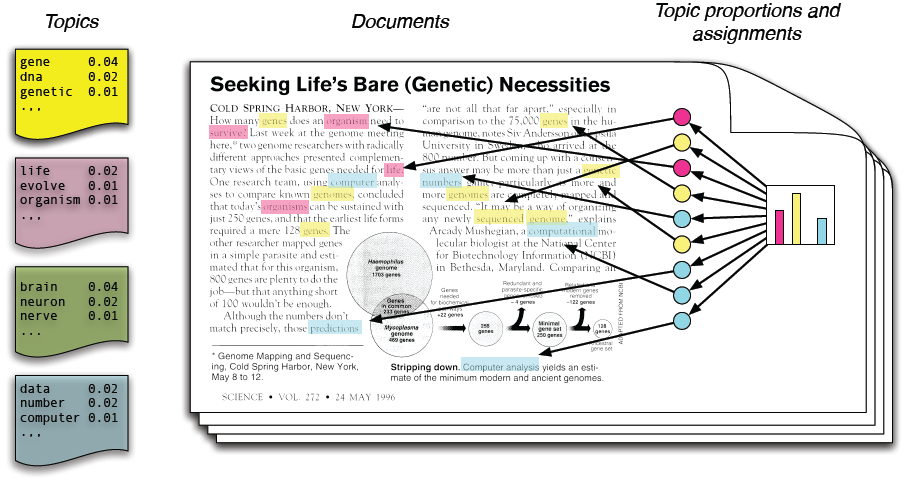
\includegraphics[width=\paperwidth]{figures/lda.png}}
\end{frame}

%
% Graphical Model and associated probability distribution
%

\begin{frame}{Graphical Model}

\vspace{0.5cm}

\noindent\makebox[\textwidth]{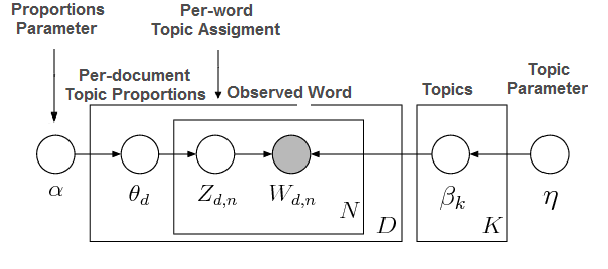
\includegraphics[width=\paperwidth]{figures/graph_model.png}}
\vspace{-0.5cm}
\Large{
$$
\prod_{k=1}^{K} p (\bm{\beta}_k|\bm{\eta}) \prod_{d=1}^{D} p(\bm{\theta}_d|\bm{\alpha})\prod_{n=1}^{N_d} p(z_{d,n}|\bm{\theta}_d)p(w_{d,n}|z_{d,n},\bm{\beta}_{1:K})
$$
}
\end{frame}

%
% Generative process
%

\begin{frame}{Generative Process}

Formally, LDA assumes the following generative process for each document $\mathbf{w}_d$:
\vspace{0.5cm}
{\large
\begin{enumerate}
\item Sample a distribution over topics $\bm{\theta}_d \sim \mathrm{Dir}(\bm{\alpha})$
\item For each of the $N_d$ words $w_{d,n}$ independently:
\begin{enumerate}
{\large
\item Draw a topic from the distribution over topics : $z_{d,n} \sim \mathrm{Mult}(\bm{\theta}_d)$
\item Draw a word from this topic : 

$w_{d,n} \sim \mathrm{Mult}(\bm{\beta}_{z,n})$
}
\end{enumerate}
\end{enumerate}
}
\vspace{0.5cm}

Intractable posterior mean :

{\Large
$$
p(\bm{\beta}, \bm{\theta}, \mathbf{z}| \mathbf{w}, \bm{\alpha}, \bm{\eta}) = \frac{p(\bm{\beta}, \bm{\theta}, \mathbf{z}, \mathbf{w}| \bm{\alpha}, \bm{\eta})}{p(\mathbf{w}| \bm{\alpha}, \bm{\eta})}
$$
}

\end{frame}

%
% Variational EM
%

\begin{frame}{Variational EM}

\begin{align*}
\text{Intractable posterior : } && p(\bm{\theta}, \mathbf{z}| \mathbf{w}, \bm{\alpha}, \bm{\beta}) & = \frac{p(\bm{\theta}, \mathbf{z}, \mathbf{w}| \bm{\alpha}, \bm{\beta})}{p(\mathbf{w}| \bm{\alpha}, \bm{\beta})}
\end{align*}
\begin{align*}
\text{Log-likelihood : } && \log p(\mathbf{w}|\bm{\alpha,\beta}) & = \log \int \sum_{\mathbf{z}}p(\bm{\theta}, \mathbf{z}, \mathbf{w}| \bm{\alpha}, \bm{\beta}) d\bm{\theta}
\end{align*}
\begin{align*}
\text{Usual trick : } && \log p(\mathbf{w}|\bm{\alpha,\beta}) & = \log \int \sum_{\mathbf{z}} \frac{p(\bm{\theta}, \mathbf{z}, \mathbf{w}| \bm{\alpha}, \bm{\beta})q(\bm{\theta},\mathbf{z})}{q(\bm{\theta},\mathbf{z})} d\bm{\theta} \\
 && & = \mathbb{E}_q \left[ \log \int \sum_{\mathbf{z}} \frac{p(\bm{\theta}, \mathbf{z}, \mathbf{w}| \bm{\alpha}, \bm{\beta})}{q(\bm{\theta},\mathbf{z})} d\bm{\theta} \right]\\
 && & \ge \mathbb{E}_q \left[ \log p(\bm{\theta}, \mathbf{z}, \mathbf{w}| \bm{\alpha}, \bm{\beta})\right] - \mathbb{E}_q \left[q(\bm{\theta},\mathbf{z}) \right] \\
 && & = \mathcal{L}(q,\bm{\alpha}, \bm{\beta})
\end{align*}

\end{frame}

\begin{frame}{Variational EM}

\begin{align*}
\text{E-step : } && \max_{q}\mathcal{L} \Leftrightarrow \min_q \mathrm{KL} \left( q(\bm{\theta}, \mathbf{z} || p(\bm{\theta}, \mathbf{z}| \mathbf{w}, \bm{\alpha}, \bm{\beta}) \right)
\end{align*}
\begin{align*}
\text{Variational distribution : } && q(\bm{\theta}, \mathbf{z}|\bm{\gamma}, \bm{\phi}) = q(\bm{\theta}|\bm{\gamma})\prod_{n=1}^{N} q(z_n|\bm{\phi}_n)
\end{align*}
\begin{align*}
\text{New E-step : } && (\bm{\gamma}^*, \bm{\phi}^*) = \underset{\bm{\gamma}, \bm{\phi}}{\text{arg min}}\;\mathrm{KL}(q(\bm{\theta}, \mathbf{z} | \bm{\gamma}, \bm{\phi})~||~p(\bm{\theta}, \mathbf{z} | \mathbf{w}, \bm{\alpha}, \bm{\beta}))
\end{align*}
\begin{itemize}
\item Overall algorithm : 
\begin{align*}
\text{E-step : } && \bm{\phi}_{n,k} & \propto \bm{\beta}_{k, w_n} \exp\{\Psi(\bm{\gamma}_k)\} \\
&&  \bm{\gamma}_{k} & = \bm{\alpha}_{k} + \sum_{n=1}^N \bm{\phi}_{n,k} \\
\text{M-step : } && \bm{\beta}_{k,j} & \propto \sum_{d=1}^D \sum_{n=1}^{N_d} \bm{\phi}_{d, n, k}w_{d,n}^{(j)}
\end{align*}
\end{itemize}

\end{frame}

\begin{frame}{Gibbs Sampling}

\textit{Collapsed} (or \textit{Rao-Blackwellized}) Gibbs sampling :
\begin{itemize}
\item $\bm{\theta}_d$ and $\bm{\beta}_k$ can be computed using only $z_{d,n}$.
\item We sample $z_{d,n}$ from posterior $p(z_n|\mathbf{z}_{\neg n}, \bm{\alpha}, \bm{\eta}, \mathbf{w})$.
\end{itemize}
\vspace{0.5cm}
Developed posterior in terms of counts :
\vspace{-0.2cm}
$$
p(z_n=k|\mathbf{z}_{\neg n}, \mathbf{w}) \propto \frac{n_{\neg n,k}^{(w_n)} + \bm{\eta}_n}{\sum_{n'=1}^{V}\left( n_{\neg n, k} ^{(w_{n'})} + \bm{\eta}_{n'}\right)}\frac{n_{\neg n, k} ^{(\mathbf{w}_n)} + \bm{\alpha}_k}{\sum_{k'=1}^{(K)} \left( n_{\neg n, k'} ^{(\mathbf{w}_n)} + \bm{\alpha}_{k'} \right) }
$$

Computation of parameters :

$$
\bm{\beta}_{k,n} = \frac{n_k ^{(w_n)} + \bm{\eta}_{t}}{\sum_{t=1}^{V} n_k ^{(t)} + \bm{\eta}_{t}}
\qquad
\bm{\theta}_{d,k} = \frac{n_m ^{(k)} + \bm{\alpha}_k}{\sum_{k=1}^{K} n_m ^{(k)} + \bm{\alpha}_k}
$$

\end{frame}

\begin{frame}{References}

\footnotesize{
\begin{thebibliography}{99} % Beamer does not support BibTeX so references must be nserted manually as below
\bibitem[Blei, 2003]{p1} Blei, David M, Ng, Andrew Y, and Jordan, Michael I. \textit{Latent dirichlet allocation}. The Journal of Machine Learning Research, 3:993-1022, 2003.
\bibitem[Heinrich, 2005]{p2} Heinrich, Gregor. \textit{Parameter estimation for text analysis}. Technical report, vsonix GmbH + University of Leipzig, Leipzig, Germany, 2005.
\bibitem[Darling, 2011]{p3} Darling, William M. \textit{A theoretical and practical implementation tutorial on topic modeling and gibbs sampling}. In Proceedings of the 49th annual meeting of the association for computational linguistics: Human language technologies, 2011.
\end{thebibliography}
}
\end{frame}



\end{document}
